
% Andrew G. West - progress_spec.tex
% Main LaTeX file for CIS400/401 Progress Report Specification

\documentclass{sig-alternate}
\usepackage{mdwlist}
\usepackage{url}

\begin{document} 

\title{Detecting Sepsis in the Intensive Care Unit}
\subtitle{CIS400/401 Senior Design Final Report}
\numberofauthors{4}
\author{
Bryan Chiang \\ \email{brchiang@seas.upenn.edu} \\ Univ. of Pennsylvania \\ Philadelphia, PA
\and Isabel Fan \\ \email{isafan@seas.upenn.edu} \\ Univ. of Pennsylvania \\ Philadelphia, PA   
\and Insup Lee \\ \email{lee@cis.upenn.edu} \\ Univ. of Pennsylvania \\ Philadelphia, PA
\and Margaret Fortino-Mullen \\ \email{margaret.fortino-mullen@uphs.upenn.edu} \\ Hospital at Univ. of Pennsylvania \\ Philadelphia, PA}
\date{}
\maketitle


\begin{abstract}
\vspace{10pt}
\textit{Severe sepsis and septic shock are major healthcare concerns that impact patients in hospital settings. The onset of sepsis occurs rapidly, giving nurses and physicians little time to react and resulting in high mortality rates. Sepsis is especially a concern in Intensive Care Units (ICUs), where patients are already in very critical conditions and undergo operations that increase the risk of sepsis contraction. In order to improve patient care and the performance of physicians and nurses, computerized guidelines for managing sepsis that take patient vital signs to compute his or her risk of sepsis have been implemented. However, for a single patient's vital sign data, these guidelines can provide very different risk scores. Our project attempts to aid in assessing the various guidelines by creating a consolidated alert interface / research tool to compare sepsis studies by applying them to the patient data acquired from Penn Presbyterian Medical Center in Philadelphia, PA. } 
\end{abstract}

\vspace{10pt}
\section{Introduction}
\vspace{10pt}
\label{sec:intro}

Sepsis is a medical condition in which bacteria infect the bloodstream. It is caused by severe bodily infections and trauma, causing bacteria to quickly spread and enter the bloodstream. For example, deep lacerations into the stomach can introduce foreign bacteria into the cavity. With the bacteria that is already in the stomach, bleeding that occurs from these lacerations would provide openings into the bloodstream through which bacteria can enter. Sepsis is a prevalent reason for intensive care unit admittance and is also highly likely to develop in ICUs due to the severe trauma and surgical procedures that occur there. 

The preliminary symptoms of sepsis include fever, chills, decreased body temperature, dizziness, and vomiting. There are also fluctuations in the heart rate, respiratory rate, and of course blood measurements such as white blood cell count, blood saturation rate, lactate, and hemoglobin. All of these physiological responses lead to the widespread activation of the immunoproteins throughout the body. This inflammed immunological response interferes with the functioning of the bowel, kidneys, liver, lungs, and multiple other organs \cite{statins}. Sepsis left untreated can quickly lead to septic shock. Defined by a significantly high blood pressure (hypertension) or low blood pressure (hypotension), palpitations, rapid heart rate, pale extremities, and very low body temperature, septic shock causes a chain reaction of dysfunctions throughout the body and can quickly become fatal.

With a high mortality rate and occurrence in United States intensive care units, researchers and hospitals have been developing and utilizing clinical management technologies in intensive care units to better manage and more effectively treat septic patients. One of the most prominent technologies used are clinical decision support systems (CDSSs), software that incorporates medical protocols, patient physiological data, and an evaluation engine to generate evidence-based advice to clinicians. Such a medical protocol includes thresholds for particular vital signs; for example, if a patient's heart rate exceeded a set threshold of 160 beats per minute, then the system would alert a doctor or nurse to provide immediate patient care. Clinical decision support systems can be used to recommend particular drug dosages, immunization reminders, or diagnose medical issues \cite{ssc}. 

\vspace{10pt}
\section{Motivation}
\vspace{10pt}
\label{sec:motivation}

Sepsis accounts for twenty-five percent of admittances into US hospital intensive-care units \cite{epi}. Affecting about 751,000 patients annually in the United States \cite{sepsis_def}, sepsis has a 20-35 percent mortality rate and septic shock a 40-60 percent mortality rate \cite{meds}. It kills about 200,000 people per year in the United States, more than stroke, Alzheimer's Disease, breast cancer, or prostate cancer. It is the second leading cause of death in non-coronary intensive care units and the tenth leading cause of death \cite{epi}. With an aging United States population, the mortality rate from sepsis is increasing at 1.5 percent every year with the diminishing immune systems of the elderly.

The costs of sepsis care further presses the need for an accurate and consolidated implementation of a computerized sepsis protocol. Seventeen billion dollars are spent on sepsis annually in the United States. The average cost of sepsis care per patient in the United States is approximately \$25,000. This direct cost of patient care for sepsis is about six times more than the average cost of other intensive care unit patients. Without accurate and effective sepsis protocols, the costs only increase as patients begin to develop severe sepsis and septic shock, causing organ dysfunctions and failures that require more costly medical care \cite{yearbook}.

Different institutions have varying thresholds for analyzing the sepsis risk of a patient, so the assessment of a single patient across different guidelines would vary significantly. There is no widespread systemic approach to predicting sepsis across institutions that allows for agreement on an individual patient's risk of sepsis. 

Given the high mortality rate, high cost per sepsis patient, and uncertainty in diagnosing a patient, a consolidated research framework that allows for the comparison of sepsis algorithms was developed.  The framework gives researchers the ability to run data-driven analysis on the effectiveness of scoring algorithms in order to find a set of thresholds to accurately predict sepsis.

\vspace{10pt}
\section{Related Work}
\vspace{10pt}
\label{sec:related_work}

This section looks at research done in sepsis protocols, as well as in clinical decision support systems and the application and implementation of smart alarms in modern hospitals.

\vspace{10pt}
\subsection{Sepsis Protocols}
\label{subsec:protocols}
\vspace{10pt}

Arguably the most widely used sepsis protocol are the guidelines provided by the Surviving Sepsis Campaign. In 2002, the need for a standardized approach to sepsis care was recognized by the European Society of Intensive Care Medicine (ESICM), the International Sepsis Forum (ISF), and the Society of Critical Care Medicine (SCCM). In 2004, these three organizations formed and published the Surviving Sepsis Campaign (SSC) in order to create a consolidated set of guidelines for the European healthcare system. These three organizations, endorsed by eleven other professional societies, sought to apply these guidelines immediately in patient bedside management. The Surviving Sepsis Campaign Guidelines were implemented in health systems in thirty countries across Europe, South America, and the United States. The study measured the change in mortality rate and the achievement of ``bundle targets'' over a time period of two years. The study defined bundle targets as portions of the SSC guidelines grouped together in milestones so that hospitals would comply with these bundles in successive fashion \cite{ssc}. 

The use of the guidelines resulted in significant improvements in the achievement of bundle targets over time. The average mortality rate in these hospitals decreased from 37 percent to 30.2 percent over a time period of two years. The healthcare systems with decreased mortality rates had significantly higher achievements of bundle targets than other hospitals that did not achieve these targets as well, showing the cause and effect of going by the SSC guidelines and the improvements in hospital care \cite{ssc}.

At the Methodist Hospital System in Texas, the application of a sepsis protocol not only decreased the cases of death from sepsis but also improved the costs of sepsis care. The protocol was implemented, through a clinical decision support system, in the surgical intensive care unit in 2009, and the mortality rate using the protocol was 14 percent, compared to the Surviving Sepsis Campaign's mortality rate that year of 31 percent, and the previous year's mortality rate of 23 percent at the Methodist Hospital surgical intensive care unit (Figure~\ref{fig:mortality_rate}). From January 2008 to August 2011, there was a observed decline in the percent of sepsis cases that resulted in death, from 35.4 percent to 17.4 percent (Figure~\ref{fig:mortality_rate_time}). The costs of sepsis care from 2009 to 2011 was observed as decreasing from \$28,300 to \$28,124 per case at Methodist Hospital \cite{methodist}.

\begin{figure}
	\begin{center}
		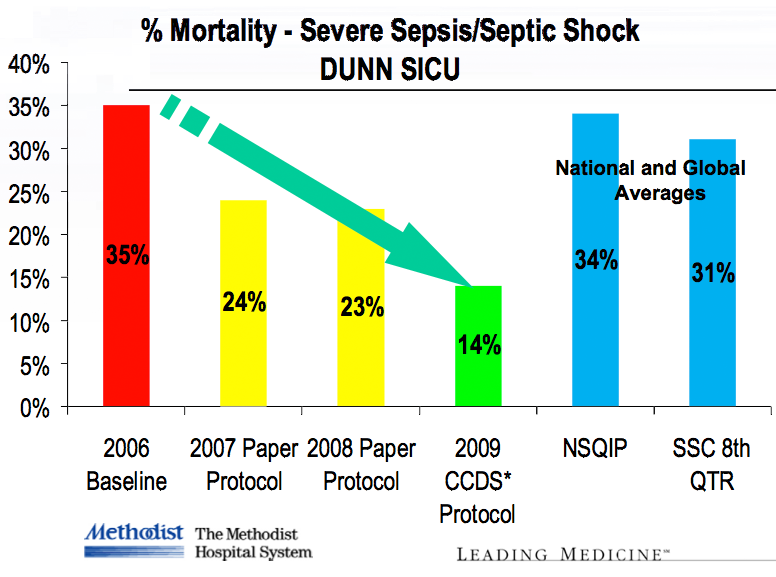
\includegraphics[width=1.0\linewidth]{methodist1.png}
	\end{center}
	\caption{Mortality rate comparison for different protocols}
	\label{fig:mortality_rate}
\end{figure}

\begin{figure}
	\begin{center}
		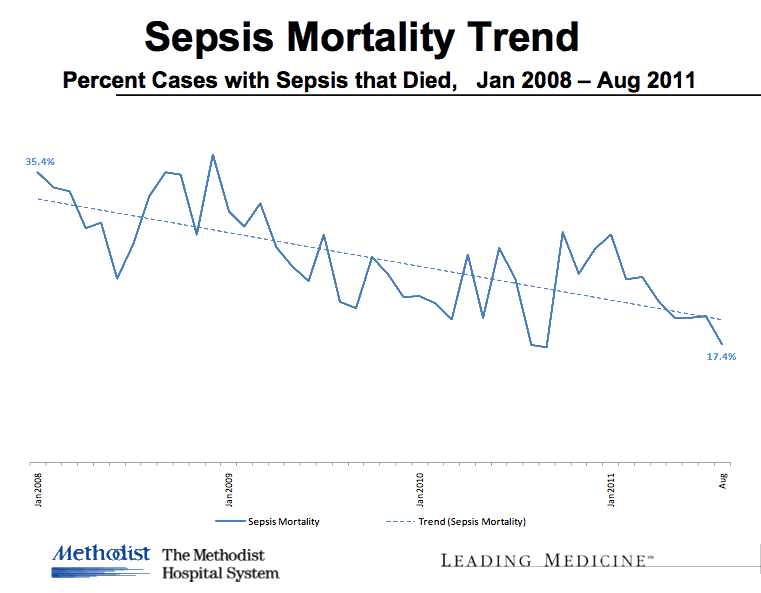
\includegraphics[width=1.0\linewidth]{methodist2.png}
	\end{center}
	\caption{Change in sepsis mortality rate over time}
	\label{fig:mortality_rate_time}
\end{figure}


\vspace{10pt}
\subsection{Clinical Decision Support Systems}
\label{subsec:cdss}
\vspace{10pt}

Clinical decision support systems can be used to diagnose patients, recommend particular drug dosages, immunization reminders, or diagnose medical issues \cite{cdss}. For this project, the focus is on clinical decision support systems that alarm when patients' conditions worsen. These alarms detect when a patient's real-time conditions exceed physiological thresholds values deemed concerns. However, having the alarm go off when only one vital sign deviates from normal does not mean that the patient has entered a critical situation. As a result, there are also instances where alarms sound off that falsely alert practitioners and result in time lost \cite{deaths}.

The University of California San Francisco assessed the effects of clinical decision support systems on physician performance. Out of a total of 68 trials, five trials tested CDSSs in their role of diagnosis. Out of these five trials, only one trial was shown to find a benefit of using a clinical decision support system. The positives were significant increases in the referral of patients for physiotherapy and a reduced risk of postoperative complications \cite{cdss}. 

The usage of alarms has not significantly improved the mortality rates and point to the alarm implementation as the weakness. First, the threshold values were set after being ``grandfathered'' through ``tradition'' as the article phrases it. In other words, the values chosen as thresholds have been based on observation through time and were not necessarily fully legitimized through quantitative proof \cite{deaths}. Second, the alarms do not go off for early signs of physiological distress, but rather when the distress is already in full effect. These smart alarms would be more reliable and effective if they were proven to detect distress before its onset \cite{deaths}.  

To improve the logic in which the alarm sounds off for a patient, research is being conducted to create smarter alarms that combine the vital signs together with patient data to more accurately alarm nurses and doctors. For instance, recent development at the University of Pennsylvania has been made for a protocol to build Smart Alarms. The first implementation of the Smart Alarm produced 53 and 59 percent drops in positive alarms without an increase in false negatives. It also doubled the amount of quiet time on the floor, making practitioners more likely to pay attention to the alarm \cite{smart_alarm}.

CDSSs also can assist in the treatment and diagnosis of diseases. This year, a team of researchers applied similar methods to diagnosing cases of acute bacterial meningitis. Using several different machine-learning models, the team managed to sift through 84 different symptoms and indicators to make the proper diagnosis with 90 percent accuracy \cite{bayes}. Existing research highlights the need for more accurate alarms that combine and analyze real-time vital signs to earlier detect a critical patient. 

\vspace{10pt}
\section{Data Collection}
\vspace{10pt}
\label{sec:data}

Sepsis data was intended to be collected from three different data sources: the Surgical and Medical ICUs at the Hospital of the University of Pennsylvania and Penn Presbyterian Medical Center.  Data from the SICU was not obtained, but the details of the intended data are discussed below.  Data from the MICU was statistically analyzed for trends in lab values but not incorporated into the smart alarm framework that was developed due to several reasons discussed below.  The data from Penn Presbyterian was ultimately used in the smart alarm framework.

\vspace{30pt}
\subsection{Surgical ICU}
\label{subsec:sicu}
\vspace{10pt}

The original intent was to use prospective data from the SICU because it was easier to monitor the patients.  With a manageable number of patients at any given time, it would be possible to keep track of which patients got septic and which ones did not.  After sepsis diagnosis, data from each classification of patients could be pulled and aggregated.  Data from the SICU comes from two sources: streaming vital sign data from the patient bedside monitors and daily lab tests from blood cultures.  The streaming vital sign data comes at a frequency of 58 seconds, whereas the lab tests are taken a few times a day.  Institutional Review Board (IRB) approval was submitted for this data, but due to HIPAA constraints, consent from each patient was required to access their data.  This level of consent was unfeasible to obtain, as the data would need to be continually collected from new patients.  The list of available data items from the SICU is listed in the Appendix.

\vspace{10pt}
\subsection{Medical ICU}
\label{subsec:micu}
\vspace{10pt}

Data from the MICU was collected from Dr. Barry Fuchs, the medical director of the MICU, who had been looking at septic patients.  The data set included 934 unique patients from July 2, 2008 - September 18, 2009.  The logic rule for this set of patients is as follows: the patient was on the general care ward, had a blood culture taken, and was transferred to the MICU in the following 2-24 hours.  The data set contains two consecutive labs for each patient that are within twelve hours of when the blood culture was drawn.  There is also information for the lab data from the last blood culture that was drawn.  The date range for the previous blood culture varies widely, ranging from within the same day to over a year.  Due to the large gap in time between some of the blood cultures, many of the patients were unusable in determining sepsis trends.  The values that were collected in this data set are listed below.
\linebreak

\noindent \textbf{Patient information:}
\begin{itemize*}
  \item Date / time of blood culture
  \item Location at order time
  \item Time of transfer to ICU
  \item Discharge time
  \item Deceased status
  \item Discharge description
\end{itemize*}

\noindent \textbf{Lab values:}
\begin{itemize*}
  \item Bicarbonate
  \item Bilirubin
  \item Creatinine
  \item Glucose
  \item International Normalized Ratio (INR)
  \item Lactic acid
  \item Platelets
  \item PO2 Arterial
  \item White blood cell count
\end{itemize*}

Due to the limited nature of this data set, only a statistical analysis was performed.  In order to do this, a few assumptions were made.  None of the classifications of the patients were included with the data set, so which patients ultimately became septic is unknown.  However, a patient being transferred from the general ward to the MICU suggests that the patient was suspected to be septic.  For the analysis, the transfer time to the MICU was considered as the reference point to compare all patients.  Ideally, the reference point would have been when each patient was diagnosed with sepsis, but this information was unavailable.  Also, since each patient only has two data points for each lab value (one from the blood culture taken at transfer and the other being the most recent blood culture before that), the patients were grouped into buckets according to the time difference between blood cultures.  The patients were grouped into five different buckets, representing time differences ranging from one to five days.  Median values for each lab result were evaluated for trends.  Trends in the data for lab values from five days before transfer to one day before transfer were evident in INR and bilirubin.

For both INR and bilirubin, median values steadily increased from five days prior to transfer to one day prior.  INR values reached 1.5, which is the threshold value for sepsis according to the Surviving Sepsis Campaign guidelines.  Bilirubin values reached 2 mg/dL, which is the stated threshold value for severe sepsis.  The trends for INR and bilirubin are shown in  Figure~\ref{fig:inr} and  Figure~\ref{fig:bilirubin} respectively.

\begin{figure}
	\begin{center}
		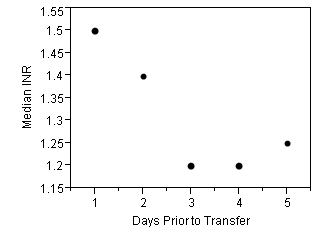
\includegraphics[width=1.0\linewidth]{INRGraph.png}
	\end{center}
	\caption{Median INR values before MICU transfer}
	\label{fig:inr}
\end{figure}

\begin{figure}
	\begin{center}
		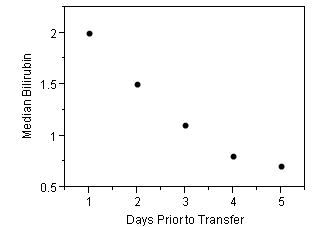
\includegraphics[width=1.0\linewidth]{BilirubinGraph.png}
	\end{center}
	\caption{Median Bilirubin values before MICU transfer}
	\label{fig:bilirubin}
\end{figure}

\vspace{10pt}
\subsection{Penn Presbyterian Medical Center}
\label{subsec:presby}
\vspace{10pt}

Data from Penn Presbyterian Medical Center was collected by a sepsis study group from patients in the month of October 2011.  The data set includes 1254 unique patients, each of which has been de-identified of personal information and newly identified by a unique ID number.  For each patient, there is basic information and information for six vital signs.  The number of vital signs depends on the length of stay for each patient, which varies.  The patient information and six vital signs collected are listed below.
\linebreak

\noindent \textbf{Patient information:}
\begin{itemize*}
  \item Hospital
  \item Emergency room time (if applicable)
  \item Arrival time
  \item Admission time
  \item First ICU time (if applicable)
  \item Final location
  \item Discharge time
  \item Hours to the ICU (if applicable)
  \item Deceased status
  \item Rapid Response Team (RRT) Call time (if applicable)
  \item Age
\end{itemize*}

\noindent \textbf{Vital signs / lab values:}
\begin{itemize*}
  \item Heart rate
  \item Lactate
  \item Respiratory rate
  \item Systolic blood pressure
  \item Temperature
  \item White blood cell count
\end{itemize*}

Similar to the MICU data, classifications for whether the patient ultimately got septic are unknown for this data set.  However, the frequency of this data set was greater than the MICU data, and was ultimately used to build the sepsis smart alarm framework.  

\begin{figure*}
	\begin{center}
		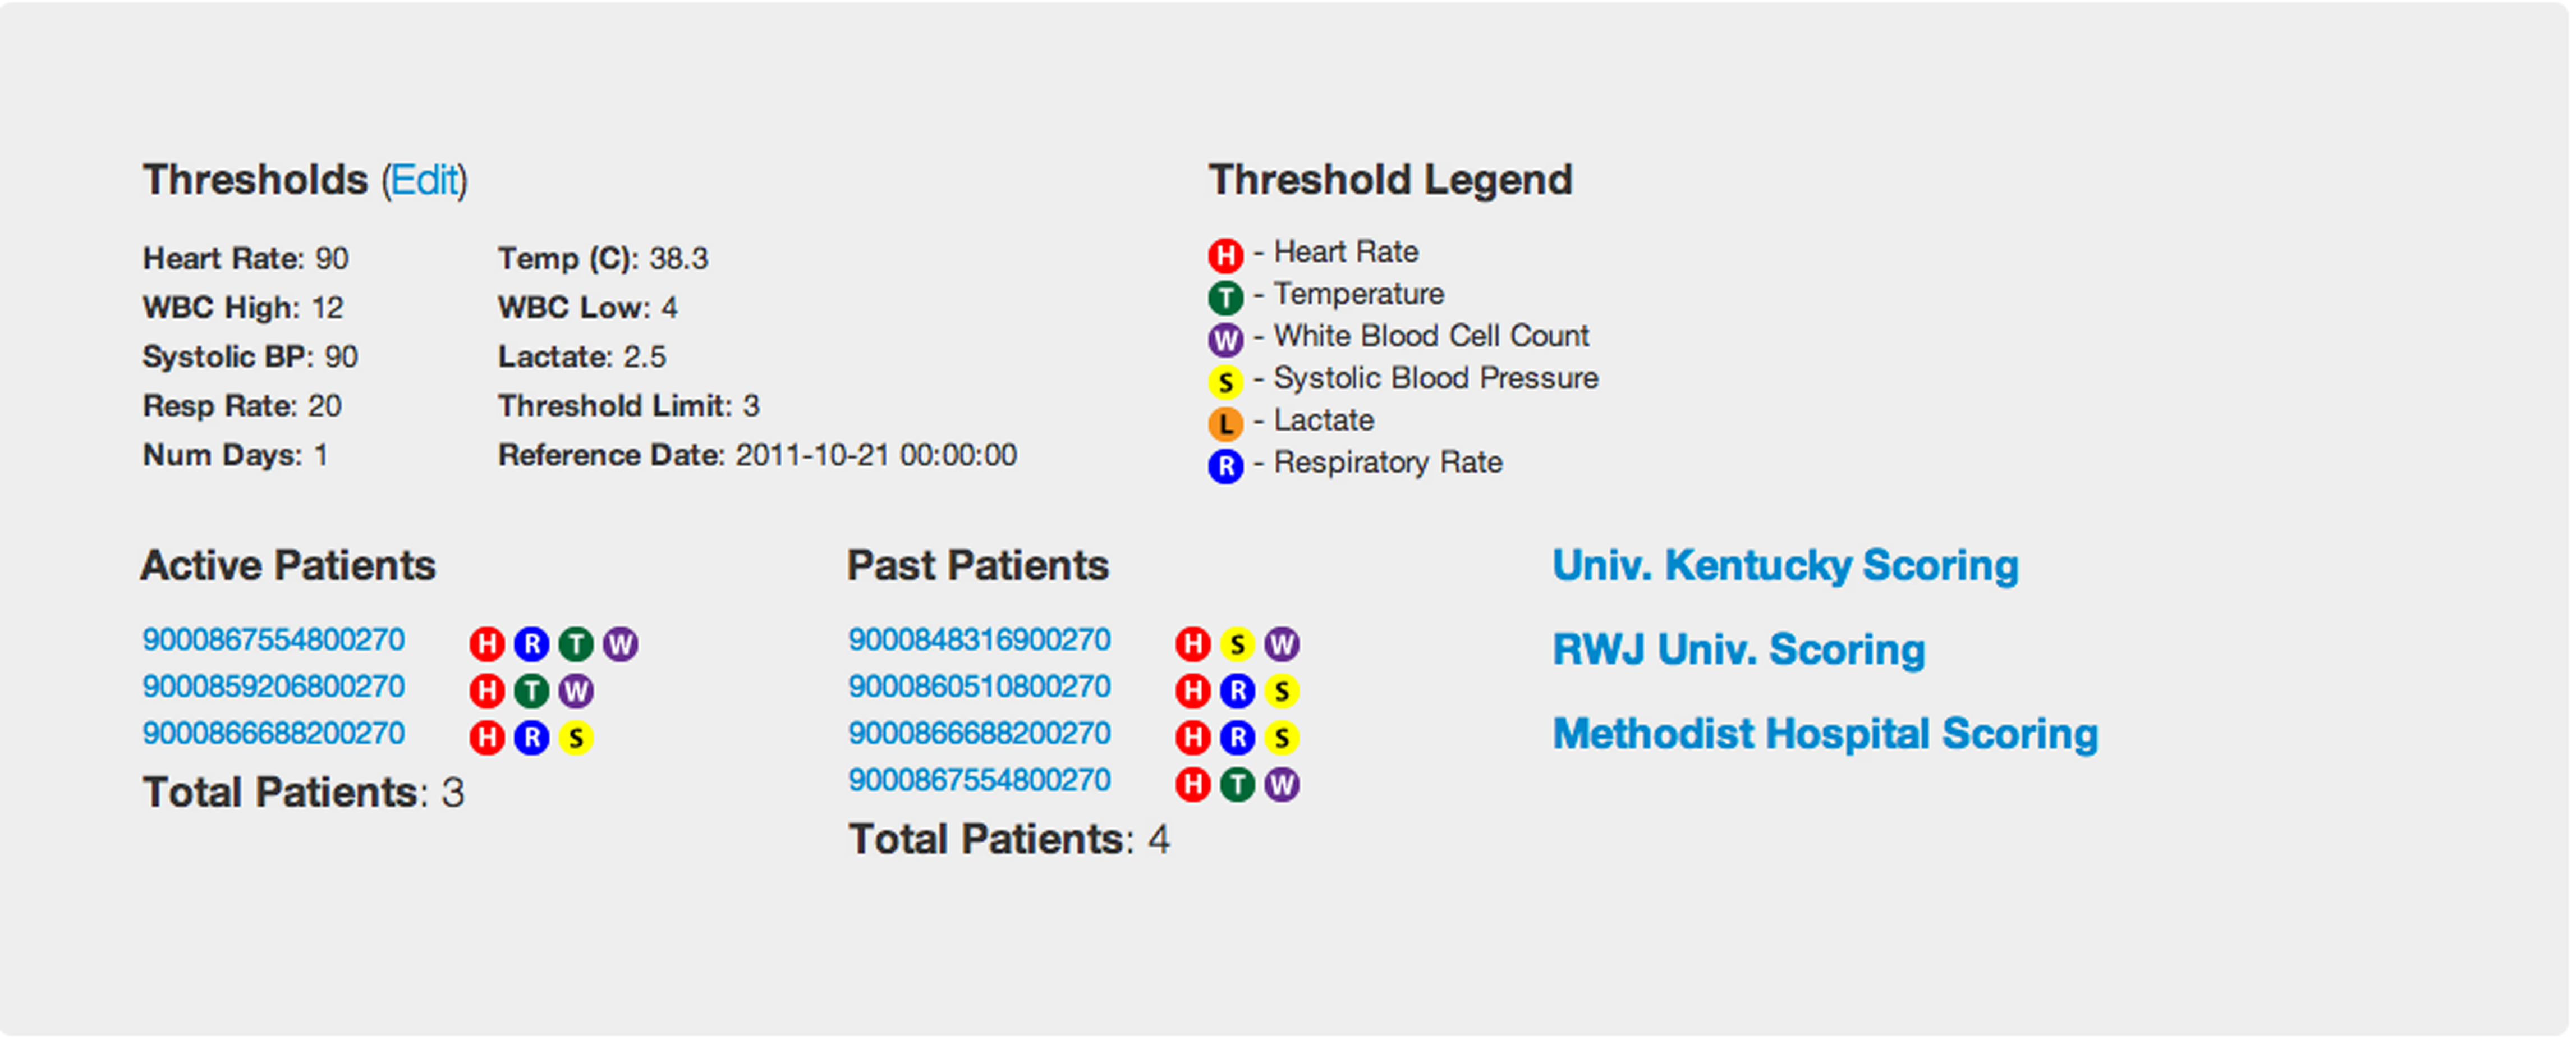
\includegraphics[width=1.0\linewidth]{home.png}
	\end{center}
	\caption{Snapshot of home screen}
	\label{fig:home}
\end{figure*}

\vspace{10pt}
\subsection{Ethics}
\label{subsec:ethics}
\vspace{10pt}

Patient privacy was definitely an ethical issue and an obstacle in the project, particularly when an inquiry into patient data access was made to the Medical and Surgical Intensive Care Units at the Hospital of the University of Pennsylvania (HUP), as well as Penn Presbyterian Hospital. The ethical issues faced largely revolved around the Health Information Portability and Accountability Act (HIPAA), which is enforced by the Office of Civil Rights of the U.S. Department of Health and Human Services to protect the privacy of individual and identifiable health information.

Requesting data access from HUP required the completion of an IRB protocol, which consisted of a complete HIPAA waiver request and authorization forms. IRB stands for Institutional Review Board, an ethics committee that monitors and reviews all research that involves patients at the HUP. The HIPAA forms asked at length what the data was going to be used for and why it was needed. Once the data was received, it was clear that great effort was made in its presentation and structure to ensure that patient confidentiality was upheld. For instance, every patient had an identification number and beyond these numbers, it was ensured that there was no other way to identify a patient. 

A potential ethical situation would be the misdiagnosis of a patient with a sepsis detection algorithm.  Relying on a computerized sepsis alert inherently poses risks, as the detection rule may not be accurate for all patients. The misdiagnosis of a patient could result in a nurse or doctor administering sepsis treatment for a patient who did not have sepsis, adding to the cost spent on that patient and utilizing excess physician resources to treat the condition. Additionally, if treatment is administered to a patient who is not septic, this could lead to further complications in the patient's health.  

\begin{figure}
	\begin{center}
		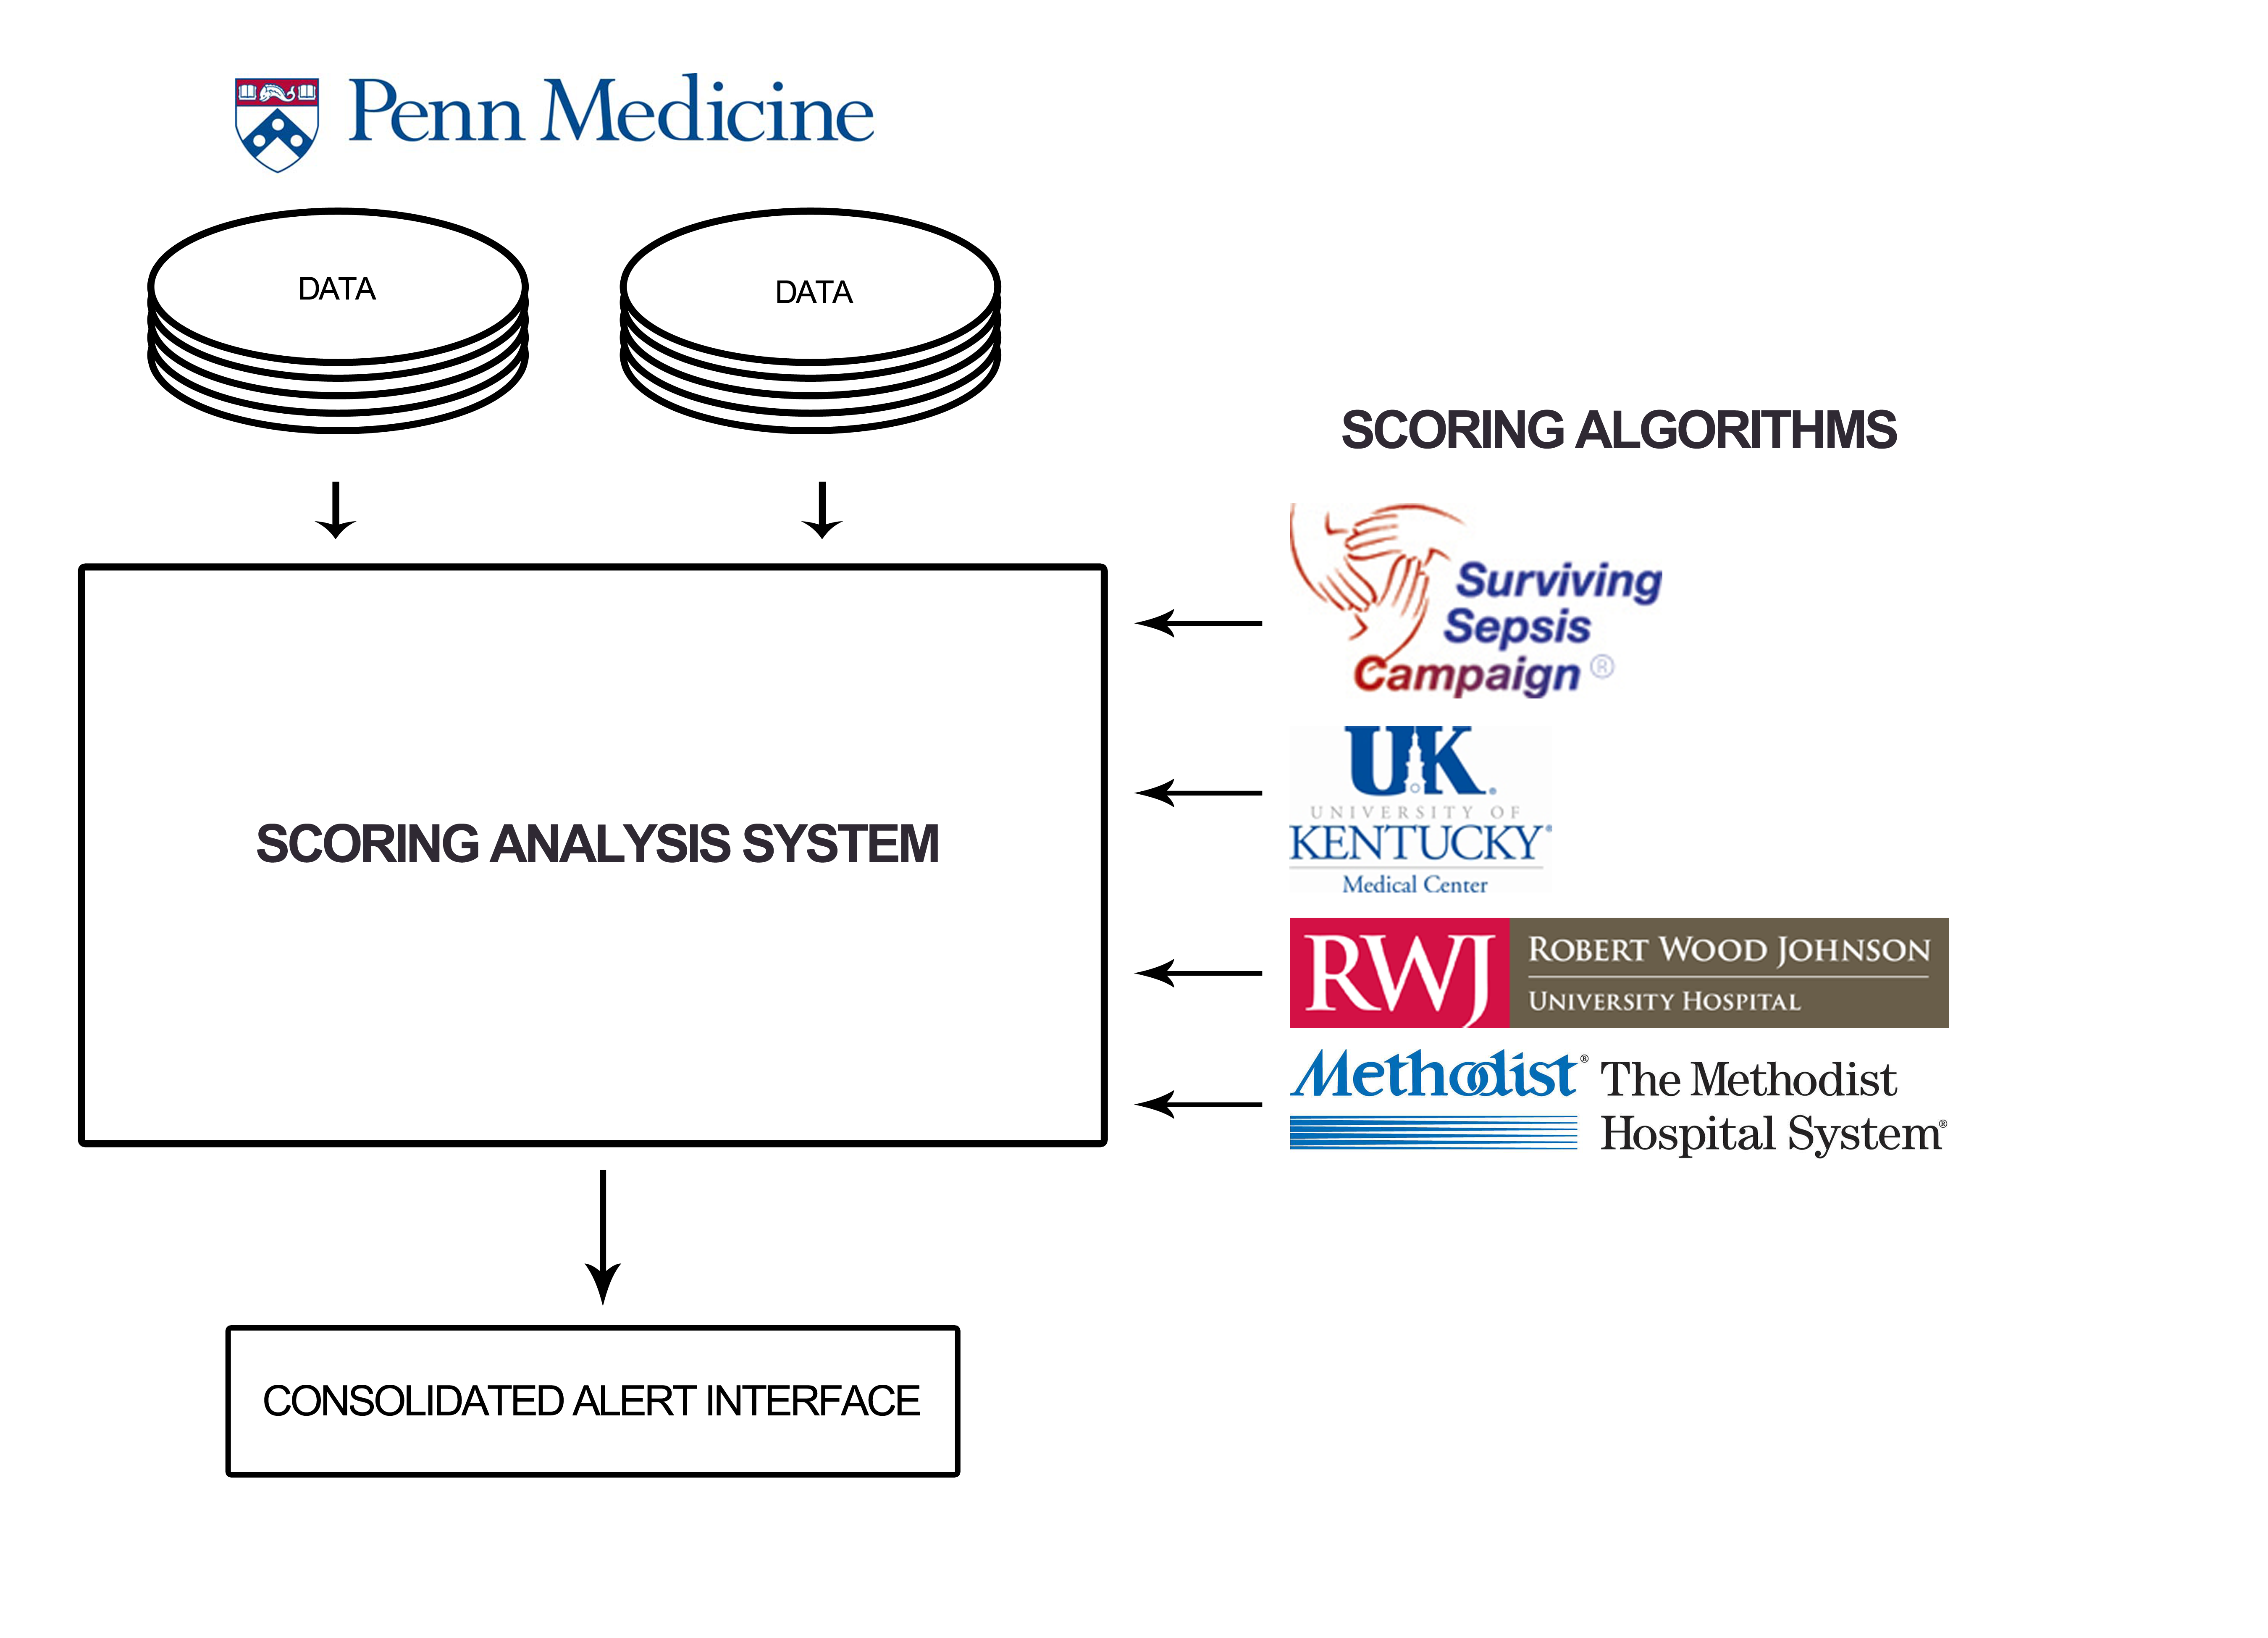
\includegraphics[width=1.0\linewidth]{FlowChart.png}
	\end{center}
	\caption{System layout}
	\label{fig:layout}
\end{figure}



\begin{figure*}
	\begin{center}
		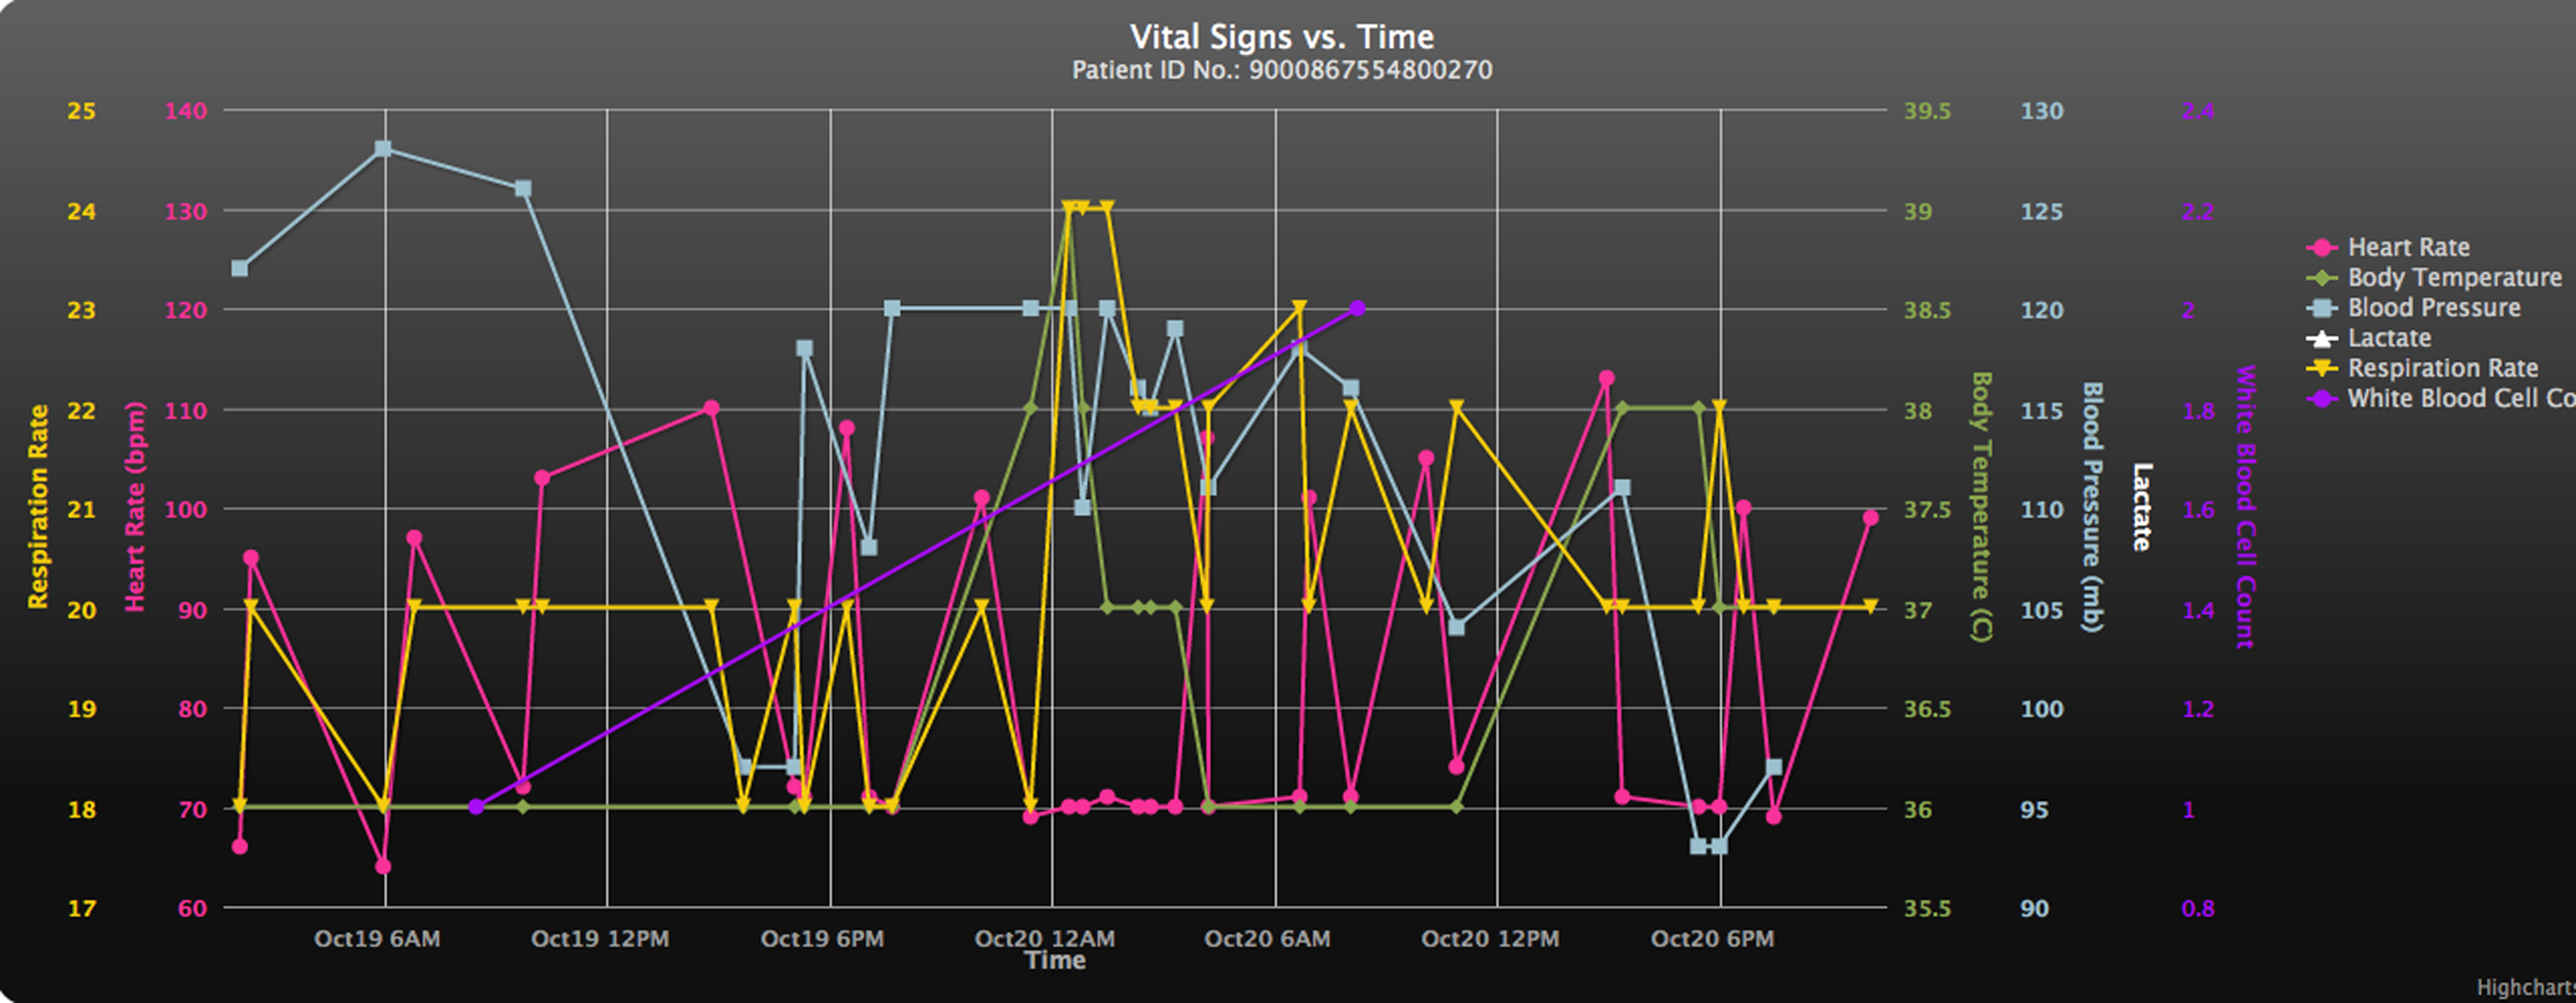
\includegraphics[width=1.0\linewidth]{patientGraph.png}
	\end{center}
	\caption{Snapshot of a patient's vital sign history graph}
	\label{fig:patient_graph}
\end{figure*}

\vspace{10pt}
\section{Smart Alarm Framework}
\vspace{10pt}
\label{sec:framework}

Since patient classifications were unknown, a smart alarm framework that could alert for suspect patients as well as serve as a research tool was built.  The layout for the framework is shown in Figure~\ref{fig:layout}.  The main functionality is to provide a set of adjustable thresholds for each vital sign collected.  Depending on the values of the thresholds and the number of thresholds that needed to be triggered, the smart alarm displays a different set of patients.  This was motivated by interviews and surveys that were conducted with nurses and physicians in the University of Pennsylvania Health System.  There was a general consensus that the vital signs provided in the Presby data set were helpful in determining whether or not a patient gets septic, but the threshold values each nurse or physician assigned varied.  Even though there are guideline values set by the Surviving Sepsis Campaign, each nurse and physician may deviate from these values.  There was also a discrepancy in the number of thresholds the nurses and physicians would look at to raise attention to that patient.  Most respondents said that three was their threshold limit.  Our framework takes into account these differences and allows the user to changes these values.

Due to the relatively small Presby data set, several assumptions were made when building the framework.  Ideally, such a smart alarm system would be used with streaming vital sign and lab data so that the information is collected in real time.  As the data is only from one month, a reference date was required to signify the current point in time.  The framework has an adjustable reference date that can be set to any time during the month of October 2011 to model how the smart alarm would look at that date.  Each patient has multiple values for each vital sign over the course of their stay at the hospital, but the date and time of each reading rarely matches up with other vital signs.  For example, respiratory rate, heart rate, systolic blood pressure, and temperature are often taken together on the same reading.  However, since white blood cell count and lactate require a blood sampling, these tests are taken less often and at different times than the other four vitals.  When trying to identify which patients trigger more than the specified level of thresholds, a time window had to be specified for those threshold trips to take place.  From the reference date, a time window of one day was used to pull the patients who met the threshold criteria.  

\vspace{10pt}
\subsection{User Interface}
\label{subsec:ui}
\vspace{10pt}

In Figure~\ref{fig:home}, the home screen of the smart alarm is displayed.  The current threshold values, number of thresholds, and reference date are displayed on top, along with a legend with each of the vital signs.  ``Active Patients'' are those who triggered more than the specified number of thresholds within one day of the reference date. ``Past Patients'' are those who triggered the set number of thresholds the day before the active patients.  Beside each of the patients, the symbols with the thresholds that were triggered are listed.  This gives the user a quick intuition into why that patient was alerted.  Clicking on a patient ID will bring the user to the patient profile page.

The user profile page contains basic information about the patient, such as their age and time admitted.  The page also provides a more detailed view of each of the vital signs so that a nurse or physician get get a better snapshot of that patient's history.  While the main page notifies which thresholds were triggered, the patient profile can show how that vital sign has been trending. A consolidated graph with each vital sign is shown in Figure~\ref{fig:patient_graph}.

\vspace{10pt}
\section{Scoring Algorithms}
\vspace{10pt}
\label{sec:scoring}

Another feature of the smart alarm framework is the ability to test different sepsis scoring algorithms.  The main scoring algorithm employed was a basic count of the number of thresholds that were triggered at the current threshold levels.  If the number of thresholds exceeded the specified limit, the patient would be alerted on the screen.  The baseline values for the thresholds were taken from the Surviving Sepsis Campaign guidelines, and the threshold values are listed in Table~\ref{tab:threshold_table}.  

\begin{table}
\renewcommand{\arraystretch}{1.5}
  \begin{tabular}{| l | l |}
\hline

{\bf Value} & {\bf Threshold}\\ \hline
Heart Rate & > 90 bpm\\ \hline
Temperature & > 38.3 $^\circ$C\\ \hline
White Blood Cell Count & >12000/$\mu$L  or <4000/$\mu$L\\ \hline
Systolic Blood Pressure & < 90 mm Hg\\ \hline
Lactate & > 2.5 mmol/L\\ \hline
Respiratory Rate & > 20 bpm\\ \hline
 \multicolumn{2}{|p{7cm}|}{\bf Rule: any three thresholds will set off the alert} \\ \hline
 \end{tabular}
	\caption{Baseline threshold values from the Surviving Sepsis Campaign guidelines}
  \label{tab:threshold_table}
\end{table}

\begin{table}
\renewcommand{\arraystretch}{1.5}
  \begin{tabular}{| l | l |}
\hline

{\bf Value} & {\bf Threshold}\\ \hline
Heart Rate & > 100 bpm\\ \hline
Temperature & < 36 or > 38.3 $^\circ$C\\ \hline
Systolic Blood Pressure & < 90 mm Hg\\ \hline
Respiratory Rate & > 24 bpm\\ \hline \hline
White Blood Cell Count & >12000/$\mu$L  or <4000/$\mu$L\\ \hline
Lactate & > 2.0 mmol/L\\ \hline
Bands & > 10\% \\ \hline
 \multicolumn{2}{|p{7cm}|}{\bf Rule: two thresholds, either two vitals or a vital and a lab value, will set off the alert} \\ \hline

 \end{tabular}
	\caption{Threshold values from RWJ University Hospital sepsis detection algorithm}
  \label{tab:rwj_table}
\end{table}

\begin{table*}
\begin{center}
\renewcommand{\arraystretch}{1.5}
  \begin{tabular}{| l | l | l | l | l | l | l | l |}
\hline

{\bf Score} & {\bf 3} & {\bf 2} & {\bf 1} & {\bf 0} & {\bf 1} & {\bf 2} & {\bf 3}\\ \hline
Heart Rate (bpm) & & < 40 & 41-50 & 51-100 & 101-110 & 110-129 & >= 130\\ \hline
Temperature ($^\circ$C) & & < 35 & & 35-38.4 & & >= 38.5 &\\ \hline
Systolic Blood Pressure (mm Hg) & < 70 & 71-80 & 81-100 & 101-199 & & >= 200 & \\ \hline
Respiratory Rate (bpm) & & < 9 & & 9-14 & 15-20 & 21-29 & >= 30\\ \hline
Age (years) & & & & & 65-74 & 75-84 & >= 85\\ \hline
BMI (kg/$m^2$) & & & < 18.5 & & 25.1-34.9 & > 35 & \\ \hline
 \multicolumn{8}{|l|}{\bf Rule: a score of 6 or greater will set off the alert} \\ \hline
 \end{tabular}
	\caption{University of Kentucky internal sepsis scoring algorithm thresholds}
  \label{tab:uk_table}
\end{center}
\end{table*}

\begin{table*}
\renewcommand{\arraystretch}{1.5}
  \begin{tabular}{| l | l | l | l | l | l |}
\hline

{\bf Score} & {\bf 0} & {\bf 1} & {\bf 2} & {\bf 3} & {\bf 4}\\ \hline
Heart Rate (bpm) & 70-109 & & 59-69 or 110-139 & 40-54 or 140-179 & <=39 or >=180\\ \hline
Temperature ($^\circ$C) & 36-38.4 & 34-35.9 or 38.5-38.9 & 32-33.9 & 30-31.9 or 39-40.9 & <=29.9 or >=41\\ \hline
Respiratory Rate (bpm) & 12-24 & 10-11 or 25-34 & 6-9 & 35-49 & <=5 or >=50\\ \hline
Systolic Blood Pressure (mm Hg) & 3-14.9 & 15-19.9 & 1-2.9 or 20-39.9 & & <1 or >=40\\ \hline
 \multicolumn{6}{|l|}{\bf Rule: a score of 4 or greater will set off the alert} \\ \hline
 \end{tabular}
	\caption{The Methodist Hospital sepsis scoring algorithm}
  \label{tab:mh_table}
\end{table*}

Additionally, scoring algorithms from the University of Kentucky Medical Center, Robert Wood Johnson (RWJ) University Hospital, and the Methodist Hospital System were tested.  The University of Kentucky used a more gradual scoring criteria, assigning a score to a range of values for each vital sign.  This sliding scale took into account the severity of the vital sign and assigned a higher score for vital signs that were further from the normal range.  Their system would alert a patient if the score was greater than six.  The RWJ University Hospital algorithm was similar to the baseline algorithm from the Surviving Sepsis Campaign Guidelines, but used a two step triggering process.  First, vital signs were tested with defined threshold values.  If any one of these four signs were triggered, lab values were tested with defined threshold values.  If any two indicators were triggered (one vital plus one lab value, or two vitals), that patient would be alerted.  The Methodist Hospital scoring algorithm is similar to that of the University of Kentucky, using a sliding scale of ranges for each value and assigning a score to each range.  A patient was alerted if the score totalled four or greater.  The algorithm constraints for the University of Kentucky, RWJ University Hospital, and Methodist Hospital are shown in Table~\ref{tab:uk_table}, Table~\ref{tab:rwj_table}, and Table~\ref{tab:mh_table} respectively.  Each of these scoring algorithms was coded into the smart alarm framework and compared to the output of the other scoring algorithms.


While the accuracy of each scoring algorithm could not be accessed, a comparison was made to see how consistent each scoring scheme was.  The reference date was changed to each day during the month of October 2011, and the outputted patients were compared for each scoring algorithm.  Each algorithm varied in sensitivity.  The RWJ University algorithm was by far the most sensitive, alerting the greatest number of patients each day.  The other three algorithms were more consistent in terms of the number of patients alerted.  On average, the four algorithms did a poor job of agreeing on septic patients.  This shows that scoring algorithms between hospitals do not agree consistently on septic patients and further research needs to be done to refine these alerts.  A summary of the number of patients alerted by each algorithm is shown in Figure~\ref{fig:num_patients} and a summary of the consistency between scoring algorithms is shown in Figure~\ref{fig:num_alerts}.

\begin{figure*}
	\begin{center}
		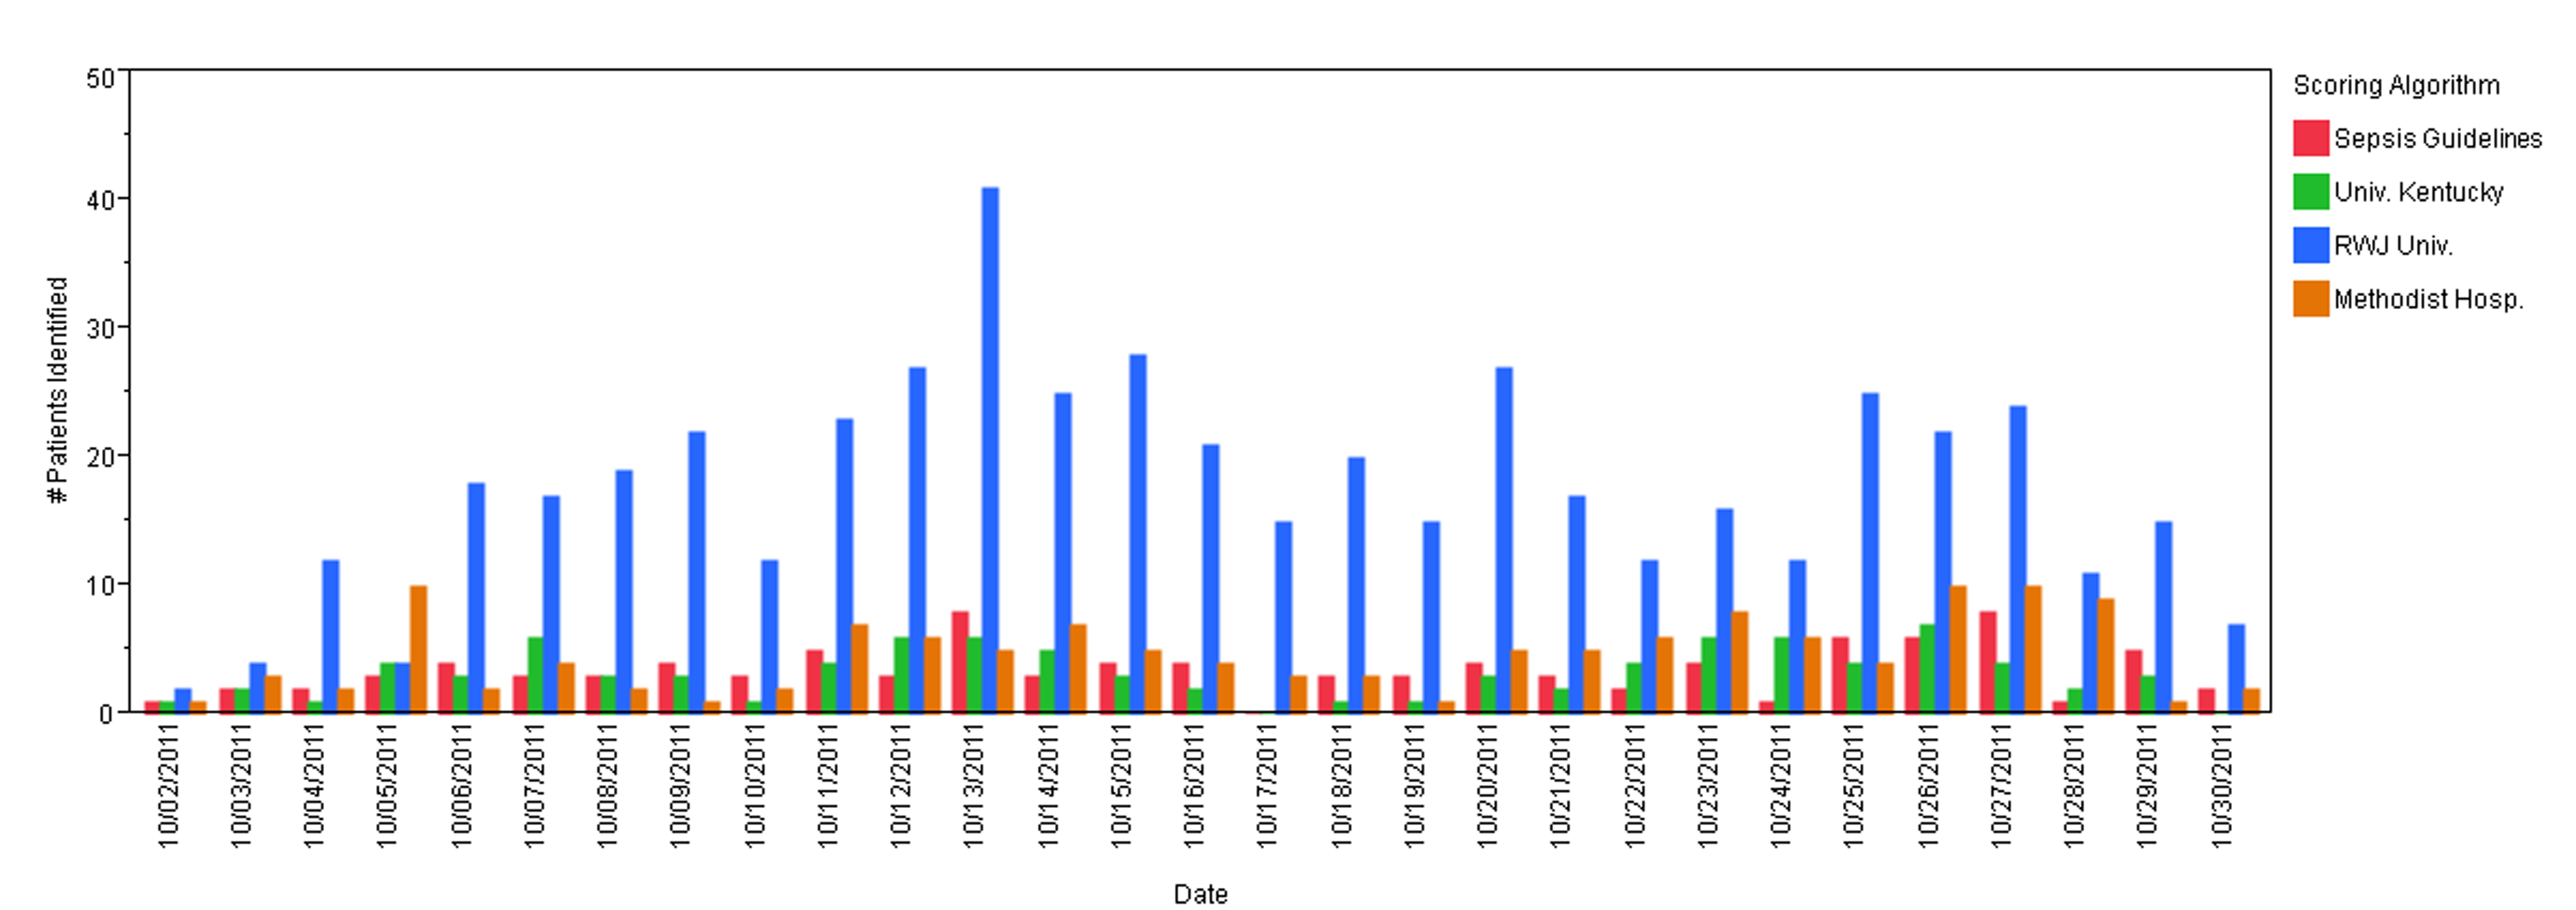
\includegraphics[width=1.0\linewidth]{NumPatientsComp.png}
	\end{center}
	\caption{Number of patients alerted by each scoring algorithm}
	\label{fig:num_patients}
\end{figure*}

\begin{figure*}
	\begin{center}
		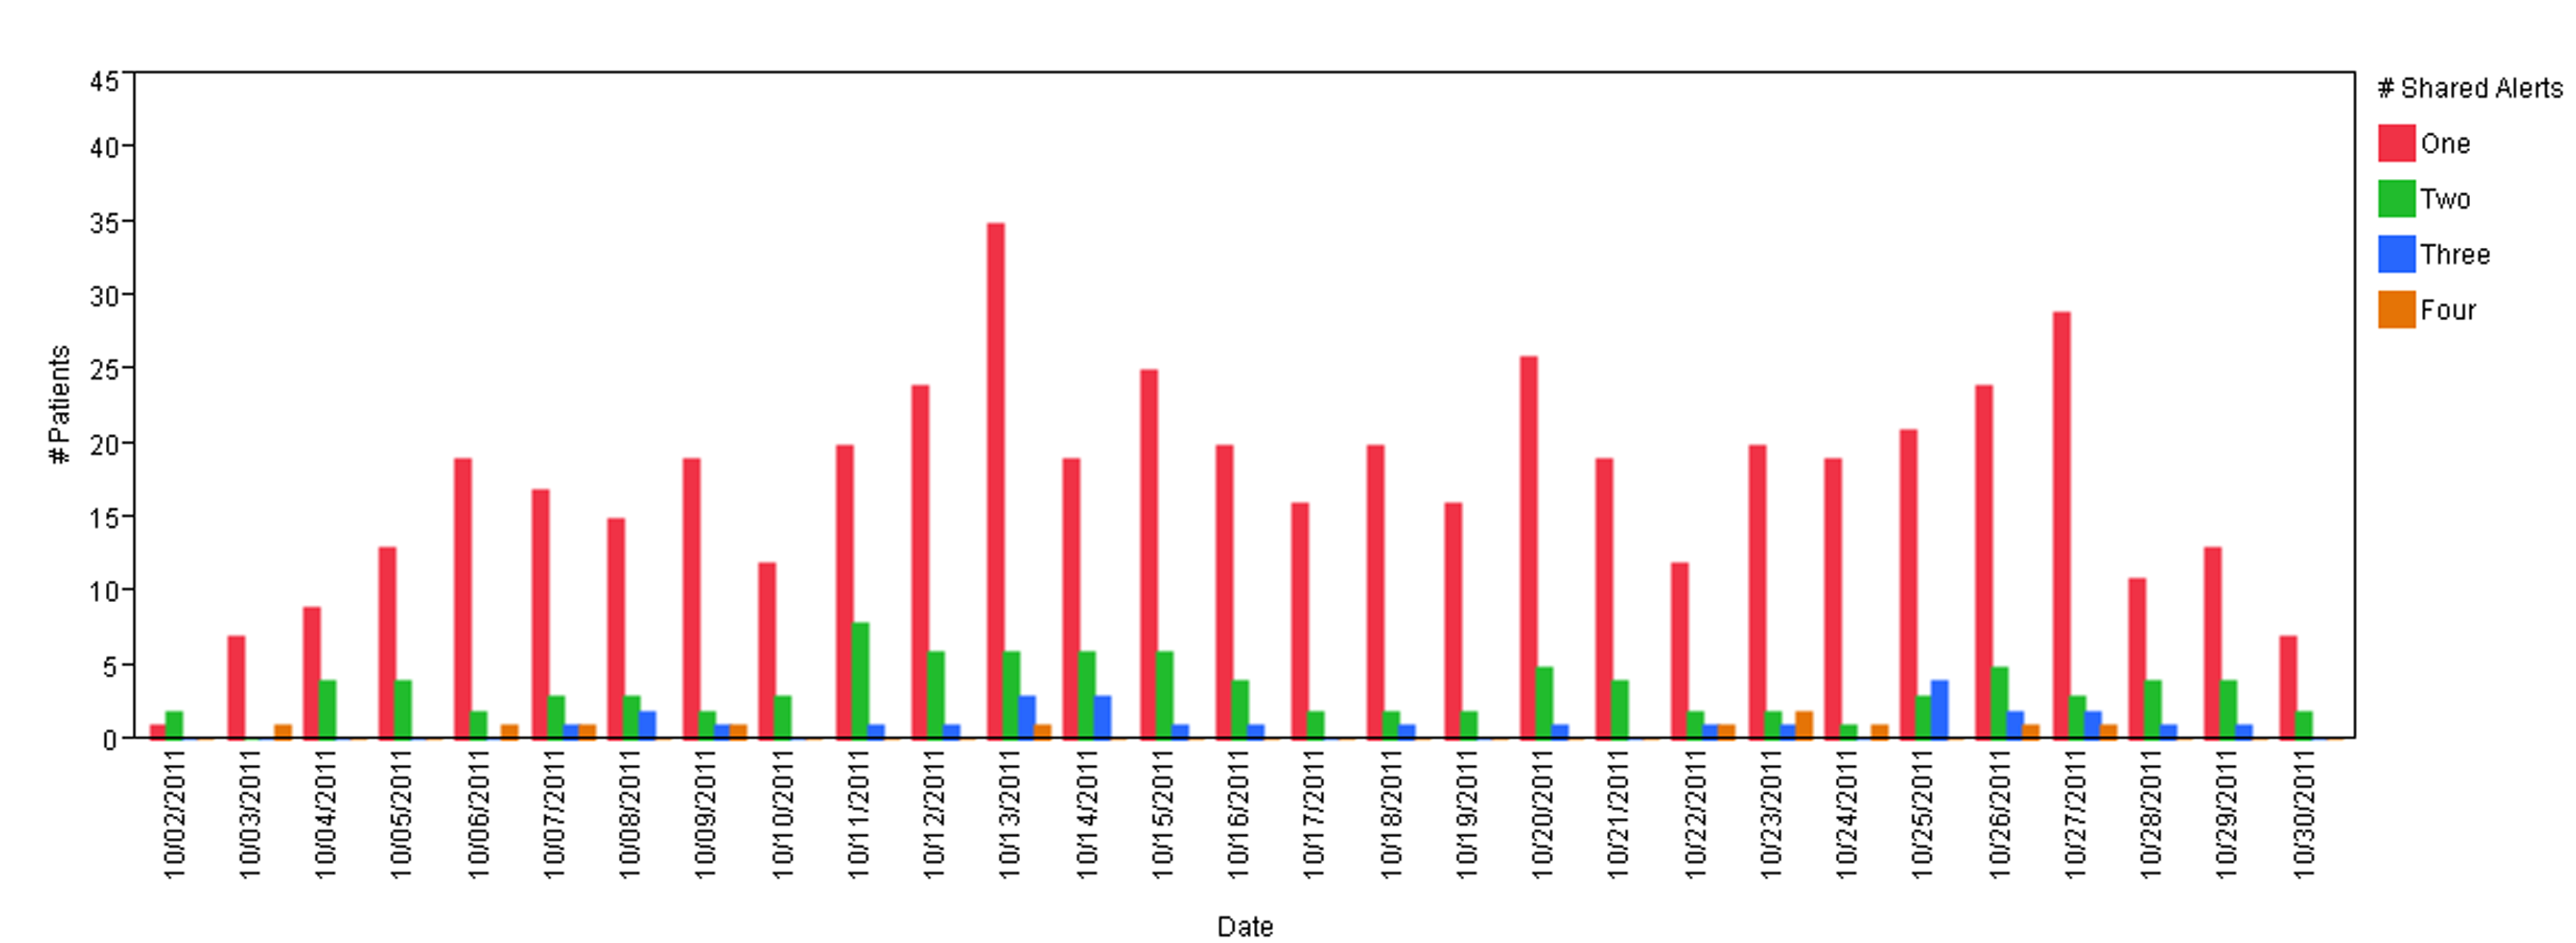
\includegraphics[width=1.0\linewidth]{ScoringComparision_Similarities.png}
	\end{center}
	\caption{Consistency of alert algorithms}
	\label{fig:num_alerts}
\end{figure*}

\vspace{10pt}
\section{Further Work}
\vspace{10pt}
\label{sec:furtherwork}

The most immediate future work would be to obtain classification labels for the patients of the Penn Presbyterian data set.  While an adjustable smart alarm framework is in place, the results and parameters cannot be evaluated without knowing which patients got septic.  Additionally, with patient labels, researchers would be able to individually alter thresholds to try to find which individual thresholds have the greatest impact on determining sepsis.  

The smart alarm framework that was created serves two purposes moving forward.  First, it acts as a research platform where the researcher can continue to alter threshold values and evaluate how accurate the detection of sepsis is.  Additionally, researchers can continue to apply scoring algorithms from other health systems to compare the relative effectiveness.  Second, as more effective scoring algorithms are developed, the framework can serve as the basis for a patient monitor alert system.  With streaming, real-time data, the home screen will constantly update as the scoring for each patient changes.  This will be useful for nurses and physicians to monitor their patients.  They can both get a broad overview of the state of their patients and have the option to click on individual patients to view specific vital signs.

\vspace{10pt}
\section{Conclusion}
\vspace{10pt}
\label{sec:conclusion}

Sepsis is a serious concern in the ICU as it has a high mortality rate and extends the length of a patient's stay.  Many hospitals currently have protocols for how to manage sepsis and different alert algorithms for detecting patients with sepsis.  While some hospitals have been able to improve sepsis detection, there is currently no effective set of thresholds that accurately predicts if a patient will become septic.  The sepsis smart alarm framework that was developed brings researchers and medical professionals one step closer to finding such a set of thresholds by supplying a data-driven method of analyzing sepsis scoring algorithms.  Using a patient data set and set of scoring algorithms, researchers can evaluate the accuracy of each algorithm and tweak threshold levels.  Ultimately, a reliable sepsis detection system will decrease the mortality rate for septic patients in the ICU and shorten the average length of a patient's stay, helping to reduce the high costs of care that a hospital faces.


\vspace{10pt}
\bibliographystyle{plain}     % Please do not change the bib-style
\bibliography{progress_spec}  % Just the *.BIB filename

\vspace{10pt}
\appendix
\section{SICU Data List}
\label{app:sicu_data}

\noindent \textbf{SICU vital sign data:}
\begin{itemize*}
  \item Heart rate \vspace{3pt}
  \item Blood pressure \vspace{3pt}
  \item Urine output \vspace{3pt}
  \item Respiratory rate \vspace{3pt}
  \item Pulsoximetry \vspace{3pt}
  \item Supplemental oxygen level \vspace{3pt}
  \item Temperature \vspace{3pt}
  \item Cardiac rhythm \vspace{20pt}
\end{itemize*}

\noindent \textbf{SICU lab work data:}
\begin{itemize*}
  \item WBC count \vspace{3pt}
  \item ANC \vspace{3pt}
  \item Bands \vspace{3pt}
  \item Hemoglobin \vspace{3pt}
  \item Hematocrit \vspace{3pt}
  \item Platelet count \vspace{3pt}
  \item Sodium \vspace{3pt}
  \item Potassium \vspace{3pt}
  \item Chloride \vspace{3pt}
  \item Bicarbonate \vspace{3pt}
  \item Bun \vspace{3pt}
  \item Creatinine \vspace{3pt}
  \item Glucose \vspace{3pt}
  \item Bilirubin \vspace{3pt}
  \item AST \vspace{3pt}
  \item ALT \vspace{3pt}
  \item Ammonia \vspace{3pt}
  \item Albumin \vspace{3pt}
  \item Amylase \vspace{3pt}
  \item Lipase \vspace{3pt}
  \item Lactate \vspace{3pt}
  \item Pt (INR)  \vspace{3pt}
  \item PTT \vspace{3pt}
  \item Fibrinogen \vspace{3pt}
  \item Sedimentation rate \vspace{3pt}
  \item C-Reactive protein \vspace{3pt}
  \item SVO2 \vspace{3pt}
  \item Venous blood gas sample \vspace{3pt}
  \item Arterial blood gas sample \vspace{3pt}
  \item Blood cultures \vspace{3pt}
  \item Sputum cultures \vspace{3pt}
  \item Urine cultures \vspace{3pt}
  \item CSF cultures \vspace{3pt}
  \item Sterile body fluid cultures \vspace{3pt}
\end{itemize*}


\end{document} 

